\documentclass[12pt,a4paper]{article}
\usepackage{amsmath, siunitx, graphicx, float, geometry, hyperref}
\geometry{margin=1in}

\title{BJT Amplifier: Temperature Dependence Study}
\author{Mainak Roy \\ University of Siegen \\ Practical Lab: Components and Circuit Technology}
\date{\today}

\begin{document}

\maketitle

\section*{Objective}
To investigate how temperature affects the linearity and gain of a BJT amplifier by analyzing the output waveform shape across a temperature sweep in LTspice.

\section*{1. Circuit Description}
The amplifier consists of a voltage divider bias using $R_1 = 1\,\mathrm{M\Omega}$ and $R_2 = 100\,\mathrm{k\Omega}$, with a BC547C transistor in common-emitter configuration. The collector is loaded with $5\,\mathrm{k\Omega}$ and powered by a $10\,\mathrm{V}$ DC supply. AC input is applied via capacitor $C_1$ with no DC offset, and output is observed through coupling capacitor $C_2$ into a $100\,\mathrm{k\Omega}$ load.

\begin{figure}[H]
    \centering
    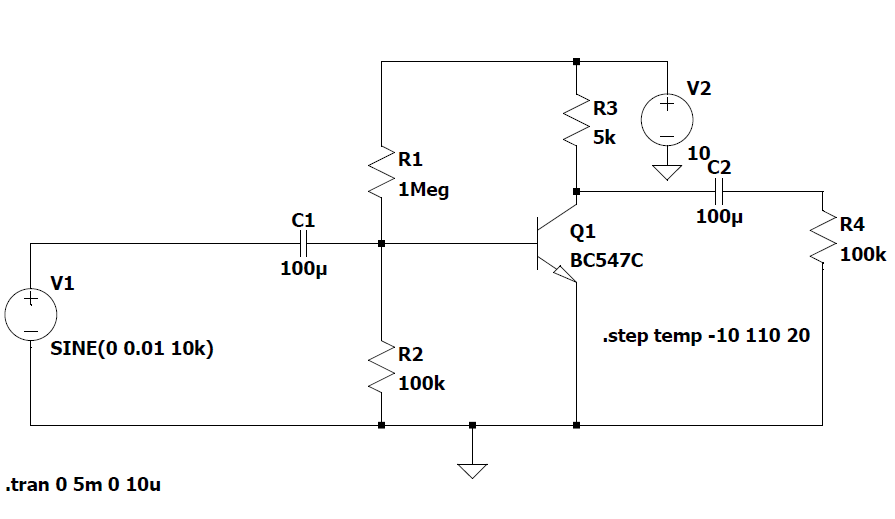
\includegraphics[width=0.85\textwidth]{schematic.png}
    \caption{LTspice schematic of the BJT amplifier with fixed bias}
\end{figure}
\vspace{1em}
\section*{2. Simulation Configuration}
LTspice simulation was configured as follows:
\begin{itemize}
    \item Transient analysis: \texttt{.tran 0 5m 0 10u}
    \item Temperature sweep: \texttt{.step temp -10 110 20}
    \item Input source: \texttt{SINE(0 0.01 10k)} (zero offset, 10~mV peak amplitude)
\end{itemize}

\section*{3. Simulation Results}
The output waveform was recorded for each temperature from \(-10\,^{\circ}\mathrm{C}\) to \(110\,^{\circ}\mathrm{C}\) in 20~\textdegree C steps. The plot below overlays all waveform results. 

At lower temperatures (e.g., \(-10\,^{\circ}\mathrm{C}\)), the output remains highly sinusoidal, indicating that the transistor operates in its linear active region. These traces typically appear as darker or colder-colored lines in the plot.

At higher temperatures (e.g., \(90\,^{\circ}\mathrm{C}\) and above), the output waveform shows visible distortion — peaks become flattened or compressed. These curves generally appear in warmer colors, such as red or magenta, depending on LTspice’s trace coloring.

\begin{figure}[H]
    \centering
    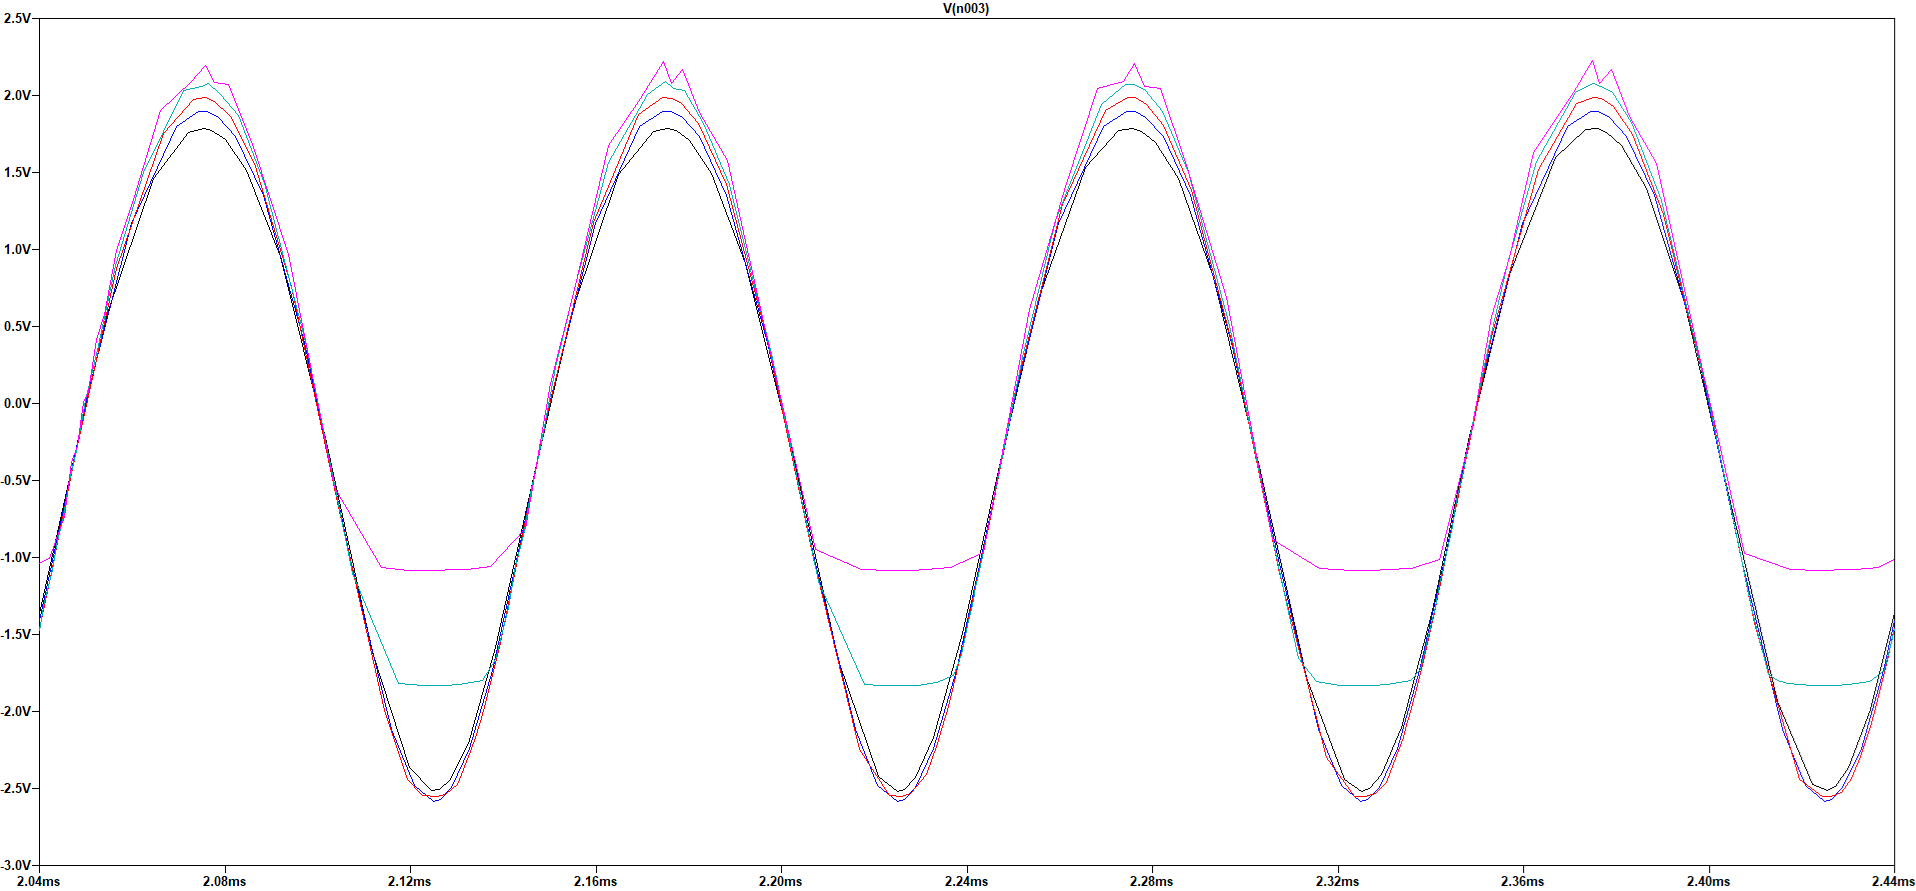
\includegraphics[width=0.85\textwidth]{waveforms_all.png}
    \caption{Output voltage waveforms for temperatures from –10~\textdegree C to 110~\textdegree C in 20~\textdegree C steps}
\end{figure}

\section*{4. Gain Estimation}
To estimate the voltage gain from a representative low-distortion waveform (e.g., at \(-10\,^{\circ}\mathrm{C}\)):

\begin{itemize}
  \item Input signal: \texttt{SINE(0 0.01 10k)} → peak amplitude = \SI{10}{\milli\volt}, so \textbf{peak-to-peak} is \SI{20}{\milli\volt} or \SI{0.02}{\volt}
  \item Output waveform (from simulation) shows approximately \SI{2.0}{\volt} peak-to-peak
\end{itemize}

\vspace{1ex}
Therefore, the AC voltage gain is calculated as:
\[
A_v = \frac{V_{\text{out, pp}}}{V_{\text{in, pp}}} = \frac{2.0\,\mathrm{V}}{0.02\,\mathrm{V}} = 100
\]
This gain value is meaningful only in the temperature range where the output remains linear. At higher temperatures, signal distortion makes such estimation unreliable.

\section*{5. Conclusion}
This experiment demonstrates that the output of a BJT amplifier is temperature-sensitive. Even with a fixed bias, variations in $V_{BE}$ and current gain with temperature cause the output waveform to shift from linear to non-linear behavior. The temperature sweep shows a clear progression from sinusoidal to distorted output, confirming the importance of temperature-stable biasing in analog amplifier design.

\end{document}
